\documentclass{article}
\usepackage{graphicx} % Nécessaire pour insérer des images
\usepackage{float}    % Pour forcer la position des figures
\usepackage{framed}   % Pour ajouter des cadres autour des images
\usepackage{listings} % Pour les exemples de code Java
\usepackage{booktabs}  % Pour une meilleure mise en forme des tableaux
\usepackage{hyperref}
\usepackage{tikz}
\usetikzlibrary{trees}

\title{Introduction au Framework Spring}
\author{Lahfari Bilal}
\date{\today}

% Paramètres pour le formatage du code Java
\lstset{ 
    language=Java,
    frame=single,
    basicstyle=\ttfamily,
    numbers=left,
    numberstyle=\tiny,
    breaklines=true,
    showstringspaces=false,
    captionpos=b,
    xleftmargin=\parindent,
    framexleftmargin=10pt,
    framexrightmargin=10pt,
    framextopmargin=5pt,
    framexbottommargin=5pt
}

\begin{document}

\maketitle

\section{Framework Spring}
\subsection{Qu'est-ce que le Framework Spring ?}

Le \textbf{Framework Spring} est un framework open-source conçu pour développer des applications d'entreprise en Java. Il simplifie le processus de développement en offrant un modèle complet de programmation et de configuration, facilitant ainsi la création d'applications robustes et évolutives.

\begin{figure}[H]
    \centering
    \begin{framed}
        
\includegraphics[width=0.8\linewidth]{images/spring_logo.png}
    \end{framed}
    \caption{Framework Spring}
    \label{fig:spring-logo}
\end{figure}

\subsection{Concepts de base de Spring}

\subsubsection{Principe de l'Inversion de Contrôle (IoC)}

\textbf{L'Inversion de Contrôle} est un principe de conception où le contrôle de la création et de la gestion des objets est transféré du code applicatif à un conteneur ou framework—dans ce cas, \textbf{le conteneur IoC de Spring}. Cela signifie que, au lieu de créer leurs dépendances, les objets dépendent du conteneur IoC pour gérer leur cycle de vie et leurs dépendances. Cela permet un code plus modulaire et maintenable, car les composants peuvent être facilement remplacés ou modifiés sans affecter les autres parties de l'application.

\begin{figure}[H]
    \centering
    \begin{framed}
        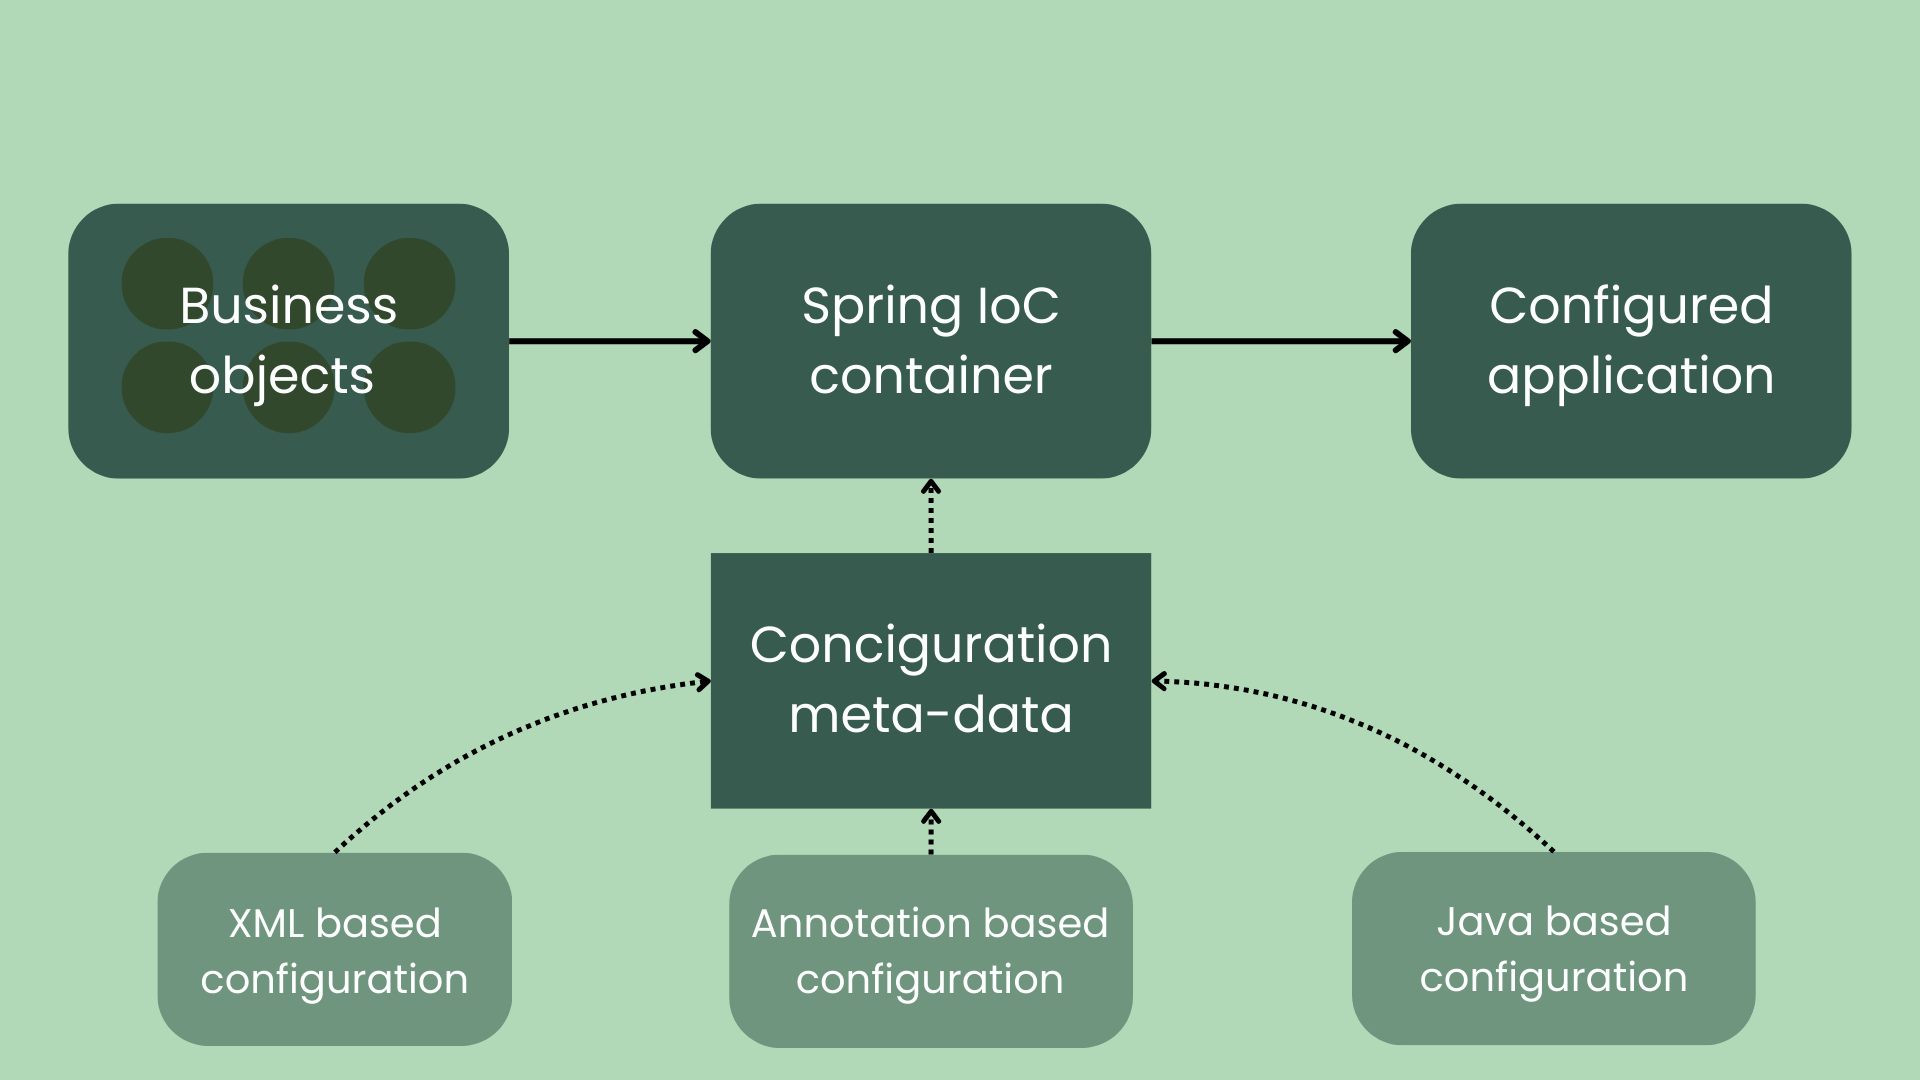
\includegraphics[width=0.9\linewidth]{images/sspring_ioc_container.png}
    \end{framed}
    \caption{Concept du conteneur IoC de Spring}
    \label{fig:spring-ioc-container}
\end{figure}

\subsubsection{Exemple d'IoC}

Pour démontrer l'Inversion de Contrôle, voici un exemple de code Java montrant une configuration Spring simple :

\begin{itemize}
    \item \textbf{Objets métiers} : POJO signifie Plain Old Java Object. Ce sont des classes Java de base qui représentent la logique métier ou les données de votre application. Elles ne contiennent aucun code Spring spécifique—ce sont de simples objets Java définissant vos données et opérations.

    \item \textbf{Conteneur IoC de Spring} : Le conteneur IoC est la partie centrale de Spring. Il est responsable de la création, de la gestion et de l'assemblage de vos objets (les POJOs) et de leurs dépendances.
    
    \item \textbf{Métadonnées de configuration} : Les métadonnées de configuration définissent les paramètres ou instructions pour le conteneur IoC. Elles indiquent au conteneur quels objets (beans) créer et comment ils doivent être connectés.
    
    \begin{itemize}
        \item \textbf{Basé sur XML} : Vous écrivez des fichiers XML pour spécifier quels beans (objets) créer et comment les connecter.
        \item \textbf{Basé sur les annotations} : Vous utilisez des annotations Java directement dans votre code pour indiquer à Spring quelles classes utiliser et comment les connecter.
        \item \textbf{Basé sur Java} : Vous utilisez du code Java pour configurer les beans et leurs dépendances, généralement via des classes annotées \texttt{@Configuration}.
    \end{itemize}
    
    \item \textbf{Application} : Une fois que le conteneur IoC lit les métadonnées de configuration et assemble les beans (POJOs), il en résulte une application entièrement configurée.
\end{itemize}

\subsubsection{Beans Spring et injection de dépendances}
\begin{itemize}
    \item \textbf{Beans Spring}  
    Un bean Spring est un objet instancié, assemblé et géré par le conteneur IoC de Spring. Ces beans représentent l'épine dorsale d'une application Spring, encapsulant la logique et les fonctionnalités de l'application. La gestion des beans inclut leur cycle de vie, leur configuration et leurs dépendances, définies via des métadonnées fournies par le développeur.

    \item \textbf{Injection de dépendances} : est un modèle de conception utilisé pour implémenter l'IoC. Cela permet au conteneur Spring de fournir les dépendances d’un objet au lieu que l'objet les crée lui-même. Cela mène à un couplage lâche entre les composants et améliore la testabilité.

\begin{figure}[H]
    \centering
    \begin{framed}
        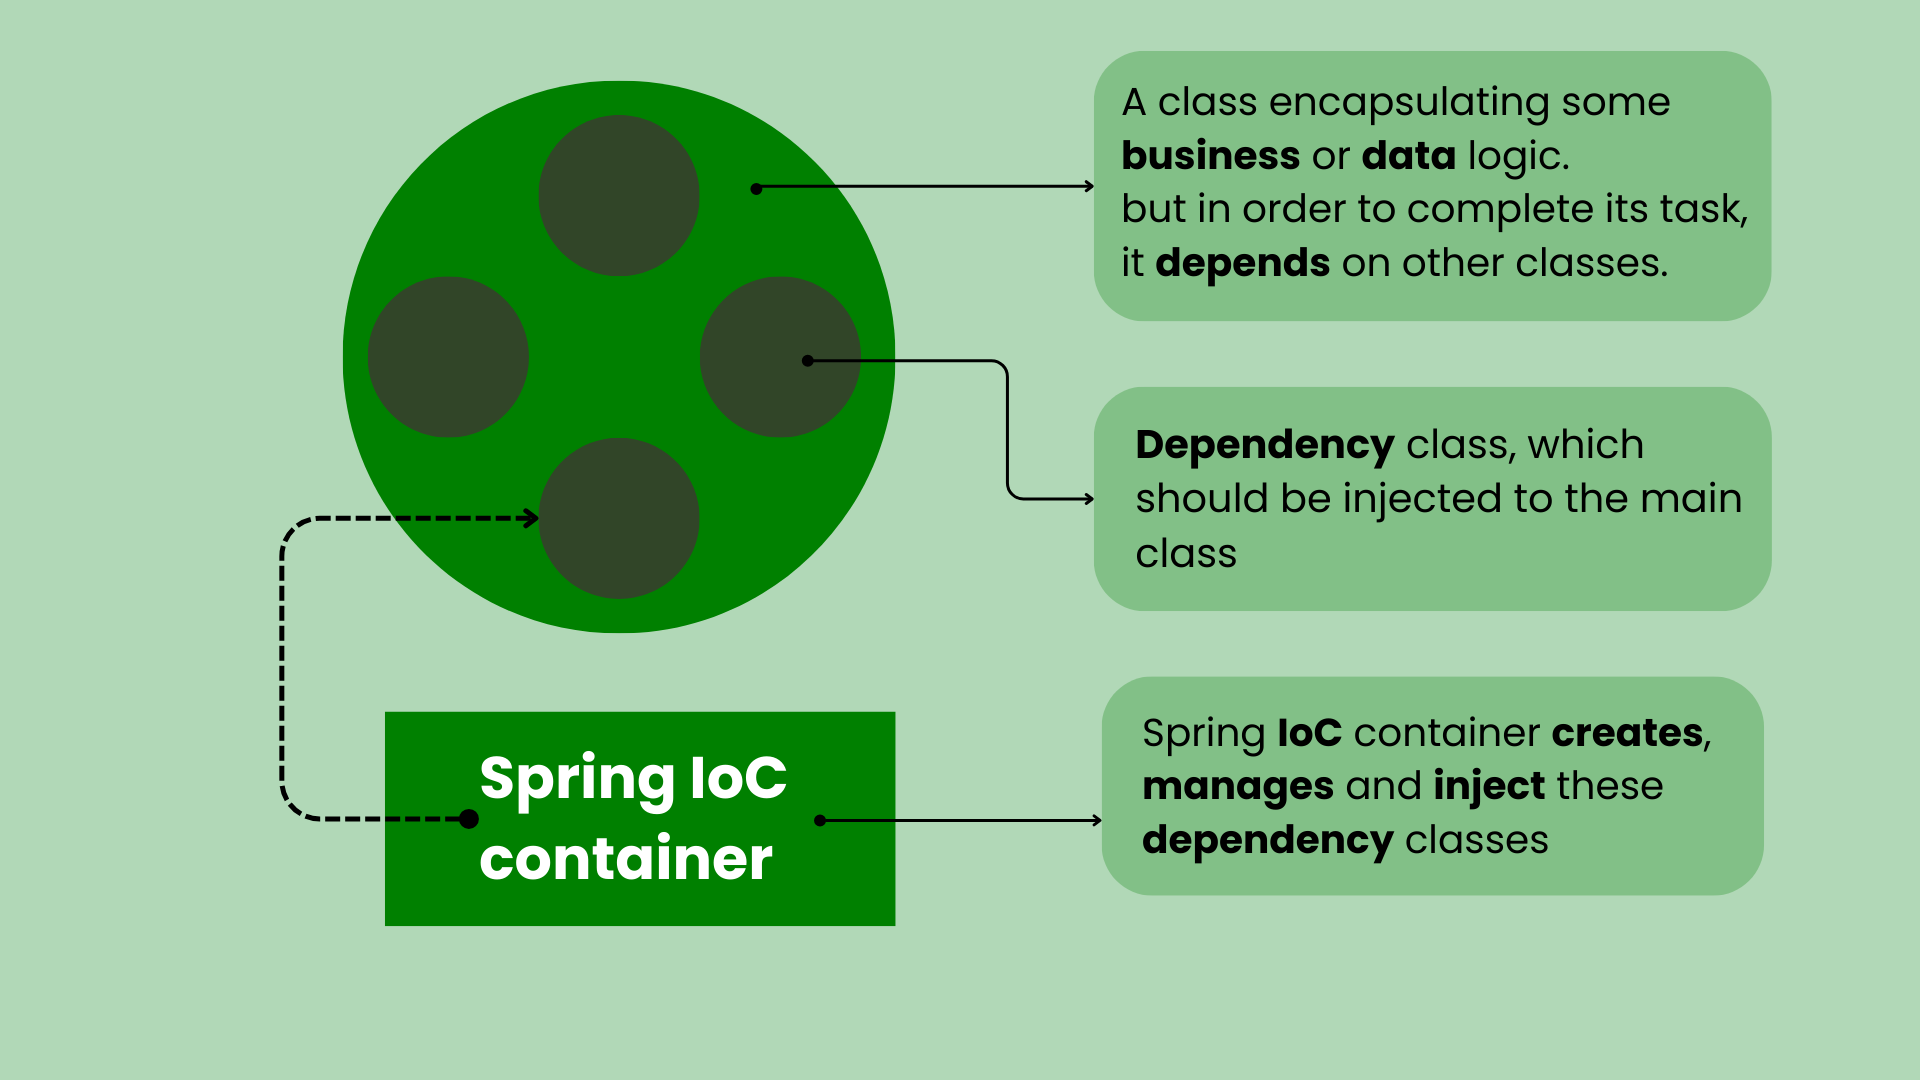
\includegraphics[width=0.9\linewidth]{images/dependency_injection.png}
    \end{framed}
    \caption{Injection de dépendances des beans}
    \label{fig:spring-ioc-container}
\end{figure}
\end{itemize}
\subsubsection{Exemples d'Injection de Dépendances}
\begin{enumerate} 
    \item \textbf{Configuration basée sur XML}\label{sec:ioc-xml-config}
    
    \item \textbf{Configuration basée sur les annotations}\label{sec:ioc-annotation-config}

    \item \textbf{Configuration basée sur Java}\label{sec:ioc-java-config}
\end{enumerate}
    
\section{Spring Boot}

\textbf{Spring Boot} est une extension du Framework Spring qui simplifie le processus de développement des applications Spring. Pour les débutants, comprendre comment Spring Boot se rapporte au Framework Spring peut aider à clarifier son objectif et ses avantages.

\begin{figure}[H]
    \centering
    \begin{framed}
        
\includegraphics[width=0.8\linewidth]{images/spring_boot_logo.png}
    \end{framed}
    \caption{Spring Boot}
\end{figure}

\subsection{Caractéristiques clés de Spring Boot} 
\begin{itemize}
    \item \textbf{Configuration automatique} : Spring Boot configure automatiquement votre application en fonction des bibliothèques incluses. Par exemple, si vous ajoutez une bibliothèque pour le développement web, il configurera un serveur web sans nécessiter une configuration extensive.

    \item \textbf{Applications autonomes} : 
    Avec Spring Boot, vous pouvez créer des applications autonomes qui fonctionnent indépendamment. Il inclut un serveur web embarqué (comme Tomcat), ce qui élimine le besoin de déployer votre application sur un serveur externe.

    \item \textbf{Dépendances de démarrage} : Au lieu de spécifier manuellement chaque dépendance dans votre fichier de configuration de projet, Spring Boot fournit des \texttt{starters} qui regroupent les bibliothèques couramment utilisées. Par exemple, \texttt{spring-boot-starter-web} inclut tout ce dont vous avez besoin pour une application web.
\end{itemize}

\section{Mise en place d'une application Spring Boot} 

\subsection{Prérequis} 

\subsubsection{Kit de développement Java (JDK) }
Vous devez avoir Java installé sur votre système. Spring Boot 3.x nécessite au moins \textbf{Java 17 ou une version supérieure}. Assurez-vous que votre version de Java est compatible avec la version de Spring Boot que vous souhaitez utiliser.

\subsubsection{Outils de build} 
Vous avez besoin d'un outil de build pour gérer les dépendances et les processus de build de votre projet. Les deux outils les plus couramment utilisés avec Spring Boot sont : 
\begin{itemize}
    \item \textbf{Maven} : La version 3.6.3 ou une version ultérieure est requise.
    \item \textbf{Gradle} : Les versions 7.x (7.5 ou ultérieures) et 8.x sont prises en charge.
\end{itemize}

\subsubsection{Environnement de développement intégré (IDE)} 
\begin{itemize}
    \item \textbf{Eclipse IDE}
    \item \textbf{IntelliJ IDEA}
    \item \textbf{Visual Studio Code}
\end{itemize}

\subsection{Créer notre premier projet}
\subsubsection{Initialisation du projet}

Il est recommandé d'utiliser Spring Initializr (\href{https://start.spring.io/}{https://start.spring.io/}) pour configurer un projet Spring Boot pour les raisons suivantes :
\begin{itemize}
    \item Génère rapidement la structure du projet et les dépendances.
    \item Permet de sélectionner les modules nécessaires (par exemple, Spring Web, Spring Data JPA).
    \item Fournit des builds préconfigurés pour Maven/Gradle.
    \item Économise du temps et simplifie le processus de configuration.
\end{itemize}

\begin{figure}[H]
    \centering
    \begin{framed}
        
\includegraphics[width=0.6\linewidth]{images/spring_init.png}
    \end{framed}
    \caption{Spring Initializr}
    \label{fig:spring-ioc-container}
\end{figure}

\subsubsection{Structure du projet}

\begin{tikzpicture}

 \tikzset{
    level 1/.style={sibling distance=50mm},
    level 2/.style={sibling distance=40mm},
    level 3/.style={sibling distance=30mm},
    level 4/.style={sibling distance=20mm},
    level 5/.style={sibling distance=10},
  }
  
  \node {MonProjetSpringBoot} 
    child { node {src} 
      child { node {main} 
        child { node {java} 
          child { node {com} 
            child { node {example} 
              child { node {demo} 
                child { node {DemoApplication.java} }
              }
            }
          }
        }
        child { node {resources} 
          child { node {application.properties} }
        }
      }
      child { node {test} 
        child { node {java} 
          child { node {com} 
            child { node {example} 
              child { node {demo} 
                child { node {DemoApplicationTests.java} }
              }
            }
          }
        }
      }
    }
    child { node {pom.xml} };
\end{tikzpicture}

\begin{enumerate}
    \item \textbf{src/main/java} : 
    \begin{itemize}
        \item Ce répertoire contient le code source principal de votre application.
        \item Il est organisé par package, suivant généralement la convention du domaine inversé (par exemple, \texttt{com.example.votreapplication}).
        \item La classe principale (par exemple, \texttt{VotreApplication.java}) contient la méthode \texttt{main} qui démarre l'application Spring Boot.
    \end{itemize}

    \item \textbf{src/main/resources} :
    \begin{itemize}
        \item Ce dossier est destiné aux fichiers de ressources dont votre application a besoin, comme les fichiers de configuration et les ressources statiques.
        \begin{itemize}
            \item \texttt{static} : Contient des fichiers statiques comme des fichiers CSS, JavaScript et images pouvant être servis directement.
            \item \texttt{templates} : Contient les templates côté serveur (par exemple, Thymeleaf ou FreeMarker) utilisés pour générer des pages web dynamiques.
            \item \texttt{application.properties} : Un fichier de configuration clé où vous définissez divers paramètres pour votre application, tels que le port du serveur, les détails de connexion à la base de données, et d'autres propriétés.
        \end{itemize}
    \end{itemize}

    \item \textbf{src/test/java} :
    \begin{itemize}
        \item Ce répertoire contient les classes de tests correspondant à votre code d'application principal.
        \item Il suit la même structure de package que \texttt{src/main/java}, permettant de garder les tests organisés à côté du code qu'ils testent (par exemple, \texttt{VotreApplicationTests.java}).
    \end{itemize}

    \item \textbf{pom.xml} :
    \begin{itemize}
        \item Il s'agit du fichier de build Maven qui gère les dépendances, les plugins et d'autres configurations du projet.
        \item Il spécifie les dépendances starter de Spring Boot que vous utilisez (comme \texttt{spring-boot-starter-web} pour les applications web) et d'autres bibliothèques nécessaires à votre projet.
    \end{itemize}
\end{enumerate}

\section{Conclusion}

Le Framework Spring et Spring Boot fournissent des outils puissants pour construire des applications d'entreprise évolutives et maintenables. En exploitant des concepts tels que l'Inversion de Contrôle (IoC) et l'Injection de Dépendances, les développeurs peuvent créer des systèmes modulaires, testables et facilement configurables. Spring Boot simplifie davantage le processus de développement grâce à sa configuration automatique, ses applications autonomes et ses dépendances préconfigurées, en faisant un choix idéal pour les applications modernes basées sur Java. Comprendre les caractéristiques clés et le processus de configuration de Spring et Spring Boot aidera les développeurs à rationaliser le développement de leurs applications et à améliorer leur productivité.


\end{document}
